\documentclass[14pt]{extreport}
\usepackage{cmap}
\usepackage[utf8]{inputenc}
\usepackage[english,ukrainian]{babel}
\usepackage{graphicx}
\usepackage{geometry}
\usepackage{listings}
\usepackage{amsmath}
\usepackage{float}
\usepackage{array}
\geometry{
	a4paper,
	left=20mm,
	right=20mm,
	top=20mm,
	bottom=20mm
}
\lstset{
	language=bash,
	tabsize=4,
	breaklines,
	keepspaces,
	showstringspaces=false,
}
\graphicspath{ {./pictures} }
\setlength{\parindent}{4em}

\newcommand\subject{Аналіз вимог до програмного забезпечення}
\newcommand\lecturer{професор кафедри ПЗ\\Грицюк Ю.І.}
\newcommand\teacher{асистент кафедри ПЗ\\Масюкевич В.В.}
\newcommand\mygroup{ПЗ-32}
\newcommand\lab{5}
\newcommand\theme{Аналіз специфікації вимог та управління ризиками розроблення програмного забезпечення}
\newcommand\purpose{Розроблення адекватного математичного методу управління ризиками розроблення ПЗ, які мають характеризувати можливі негативні наслідки їх прояву, а також збитки від подальшого функціонування ПЗ}

\begin{document}
\begin{normalsize}
	\begin{titlepage}
		\thispagestyle{empty}
		\begin{center}
			\textbf{МІНІСТЕРСТВО ОСВІТИ І НАУКИ УКРАЇНИ\\
				НАЦІОНАЛЬНИЙ УНІВЕРСИТЕТ "ЛЬВІВСЬКА ПОЛІТЕХНІКА"}
		\end{center}
		\begin{flushright}
			Інститут \textbf{КНІТ}\\
			Кафедра \textbf{ПЗ}
		\end{flushright}
		\vspace{140pt}
		\begin{center}
			\textbf{ЗВІТ}\\
			\vspace{10pt}
			До лабораторної роботи № \lab\\
			\textbf{На тему}: “\textit{\theme}”\\
			\textbf{З дисципліни}: “\subject”
		\end{center}
		\vspace{40pt}
		\begin{flushright}
			
			\textbf{Лектор}:\\
			\lecturer\\
			\vspace{10pt}
			\textbf{Виконав}:\\
			
			студент групи \mygroup\\
			Коваленко Д.М.\\
			\vspace{10pt}
			\textbf{Прийняв}:\\
			
			\teacher\\
			
			\vspace{28pt}
			«\rule{1cm}{0.15mm}» \rule{1.5cm}{0.15mm} 2023 р.\\
			$\sum$ = \rule{1cm}{0.15mm}……………\\
			
		\end{flushright}
		\vspace{\fill}
		\begin{center}
			\textbf{Львів — 2023}
		\end{center}
	\end{titlepage}
		
	\begin{description}
		\item[Тема.] \theme.
		\item[Мета.] \purpose.
	\end{description}

	\section*{Лабораторне завдання}
	Результат будь-якого програмного проекту залежить від кількості та величини ризиків недостатньої функціональності ПЗ, невиконання термінів реалізації програмного проекту, перевищення виділеного бюджету. Тому процес управління ризиками розроблення ПЗ на підставі специфікації вимог до нього (SRS) має бути однією з складових процесу управління програмними проектами.  У роботі потрібно розробити ПЗ, яка має реалізувати метод управління ризиками розроблення ПЗ з такими основними функціональними можливостями
	\begin{enumerate}
		\item має давати можливість ідентифікувати джерела появи ризиків і можливі ризики для будь-якого програмного проекту.
		\item оцінювати ризики розробити ПЗ, визначити їх пріоритет і розробити заходи із зменшення або усунення ризиків
		\item оцінювати ризики розробити ПЗ після застосування обраних заходів із зменшення або усунення ризиків, що робить можливим підібрати найкращий захід для максимального зменшення величини кожного ризику.
	\end{enumerate}
	
	\begin{figure}[H]
		\centering
		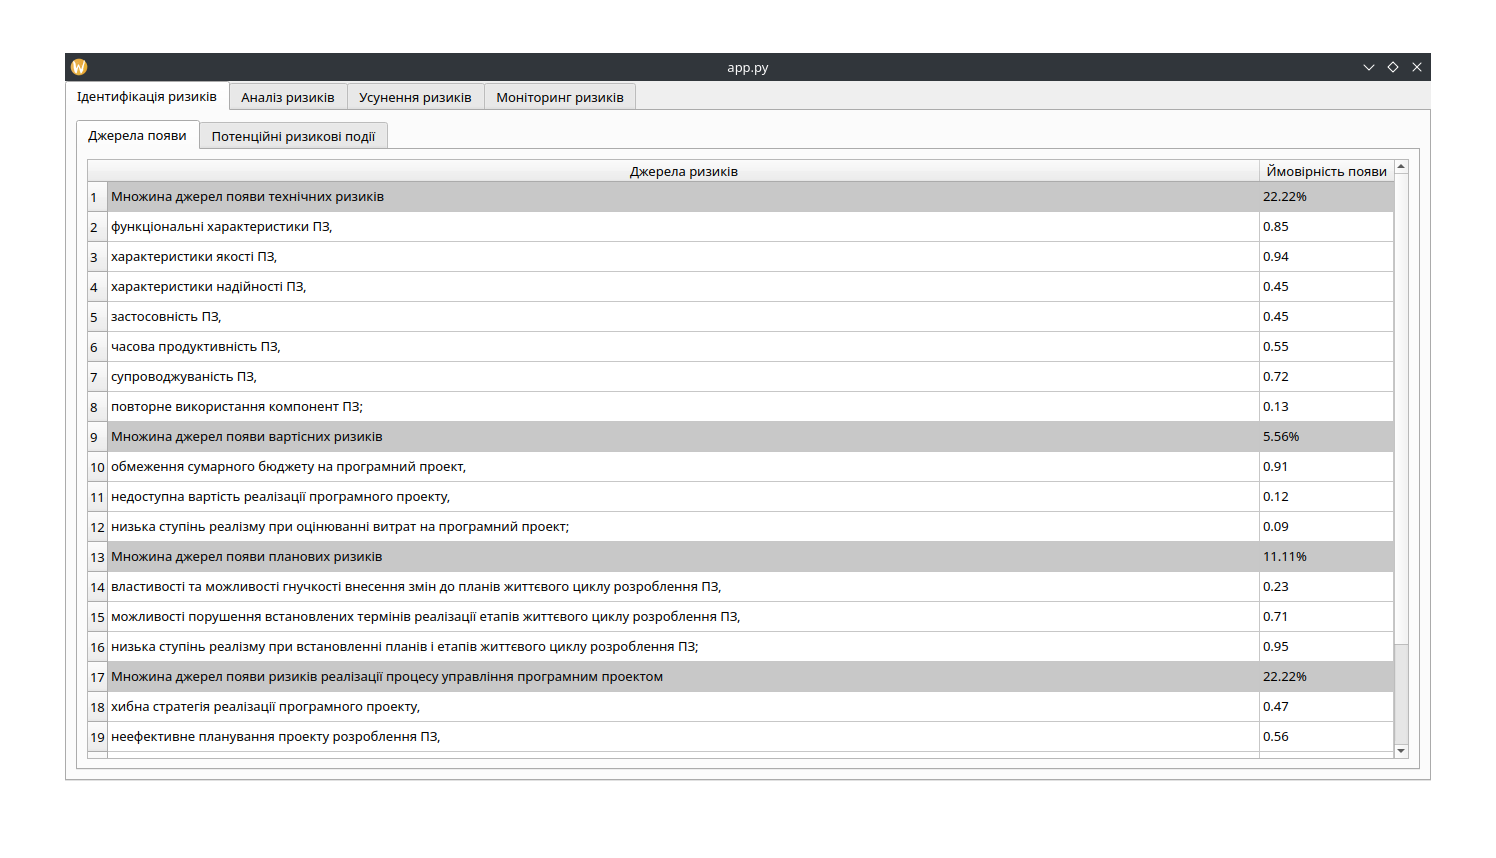
\includegraphics[scale=0.45]{1}
		\caption{Ідентифікація джерел появи ризиків}
	\end{figure}

	\begin{figure}[H]
		\centering
		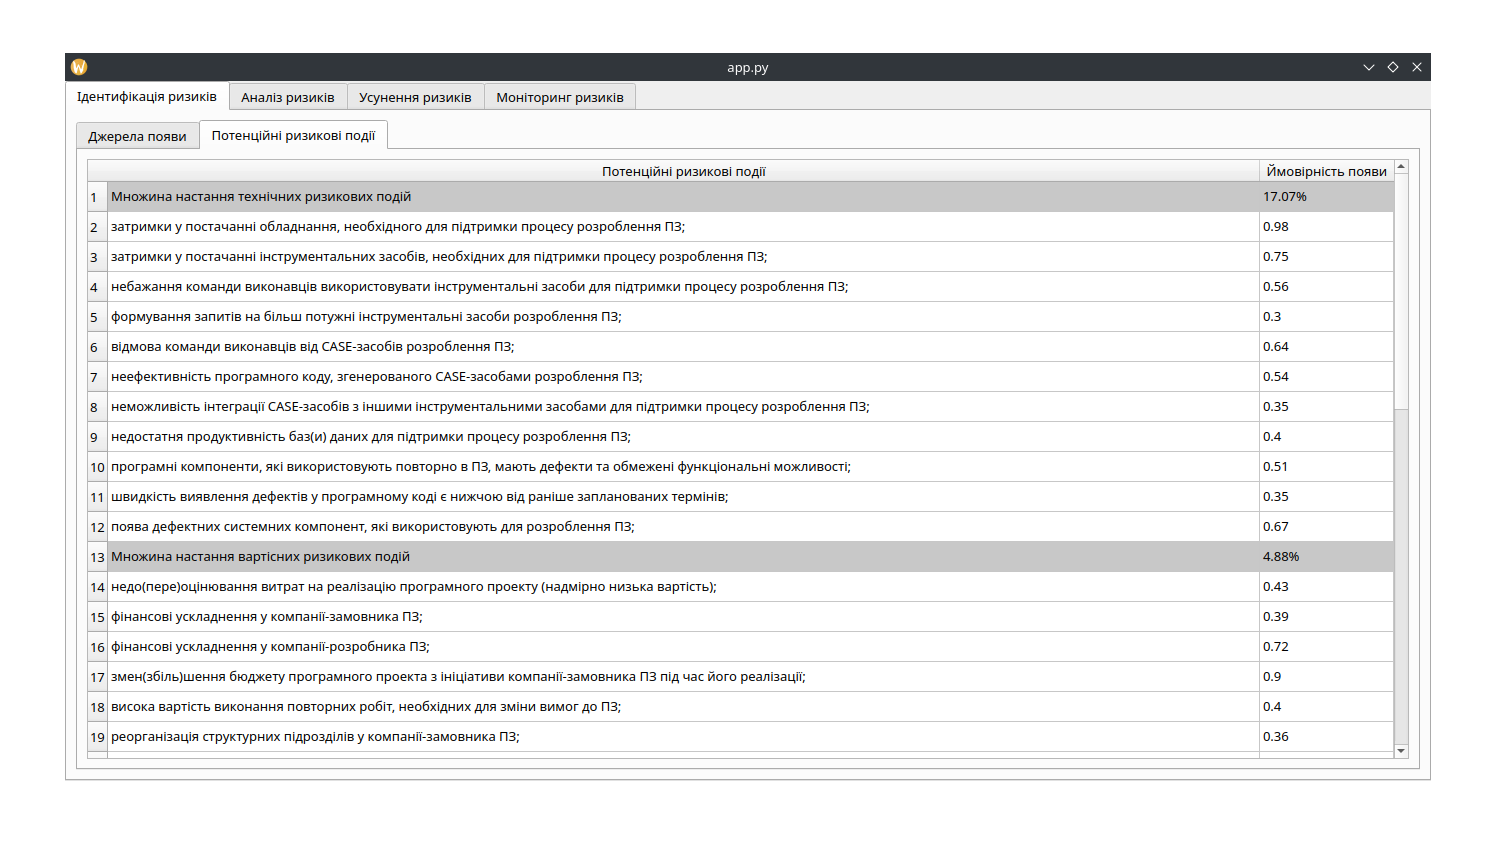
\includegraphics[scale=0.45]{2}
		\caption{Ідентифікація потенційних ризикових подій}
	\end{figure}
	
	\begin{figure}[H]
		\centering
		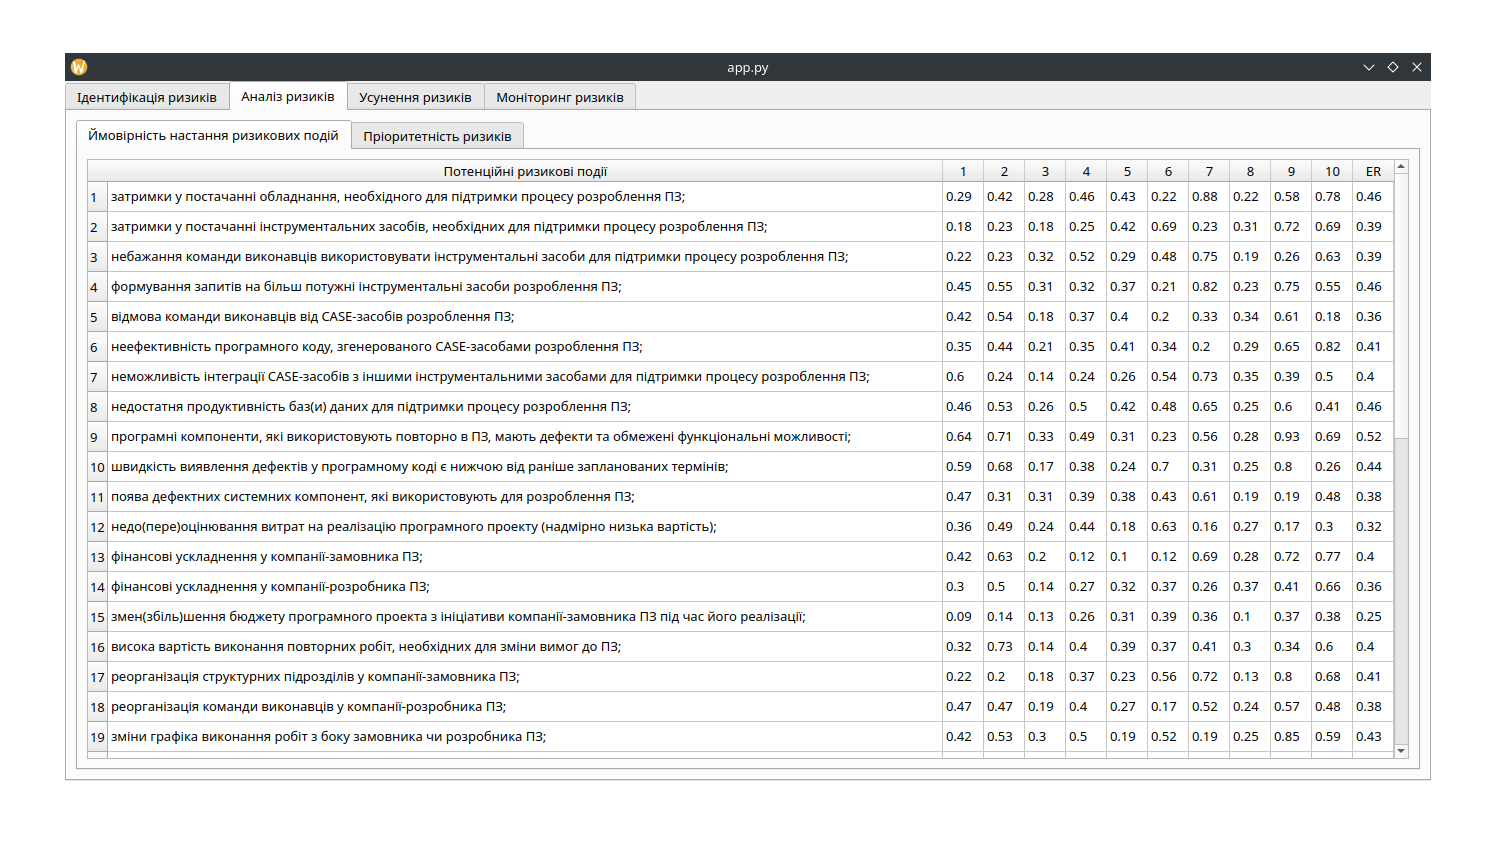
\includegraphics[scale=0.45]{3}
		\caption{Визначення ймовірності появи ризиків}
	\end{figure}
	
	\begin{figure}[H]
		\centering
		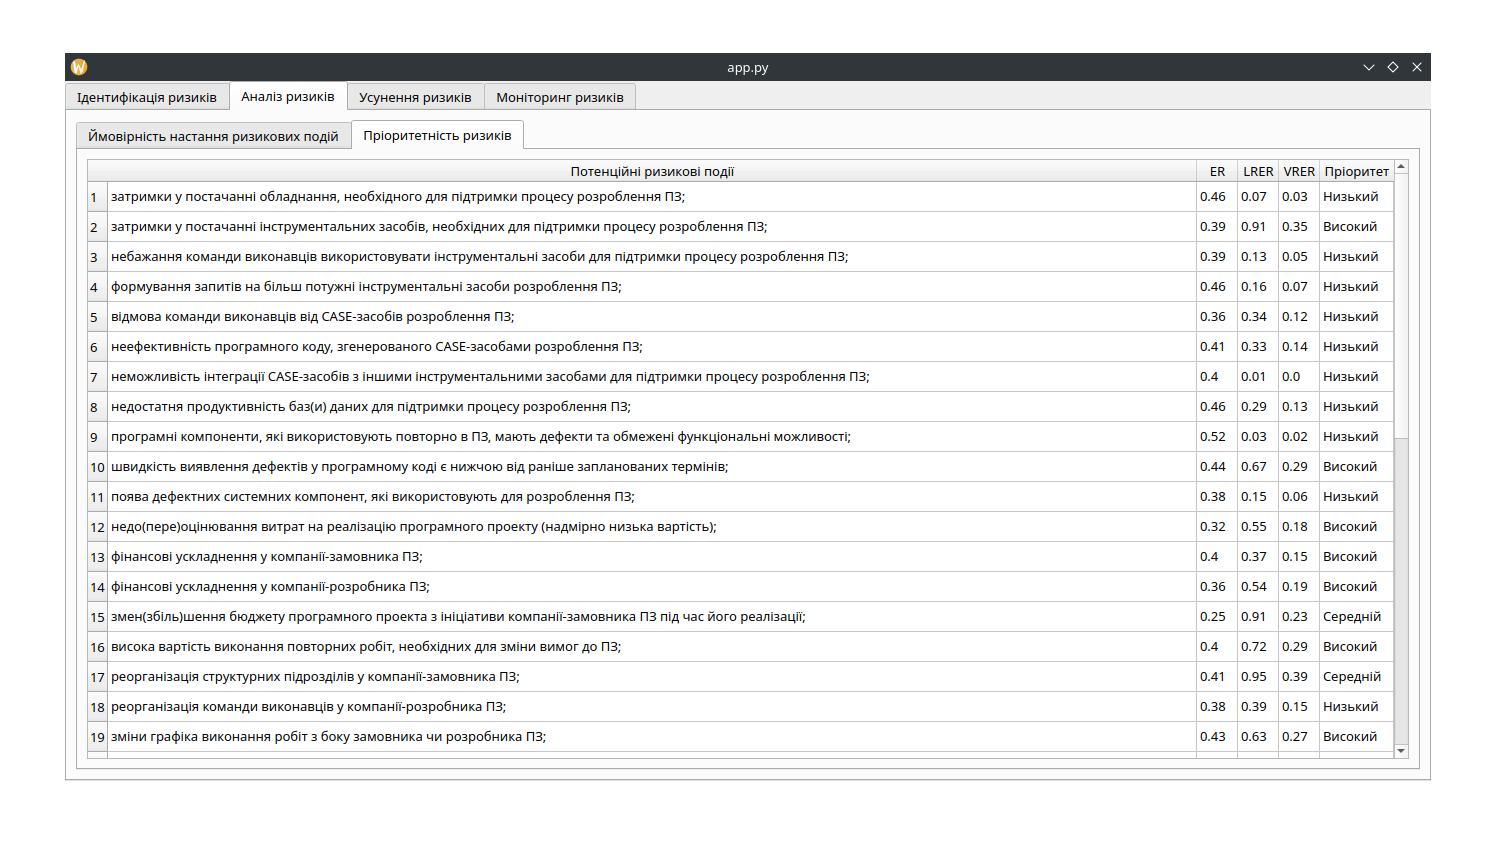
\includegraphics[scale=0.45]{4}
		\caption{Визначення пріоритетності ризиків}
	\end{figure}
	
	\begin{figure}[H]
		\centering
		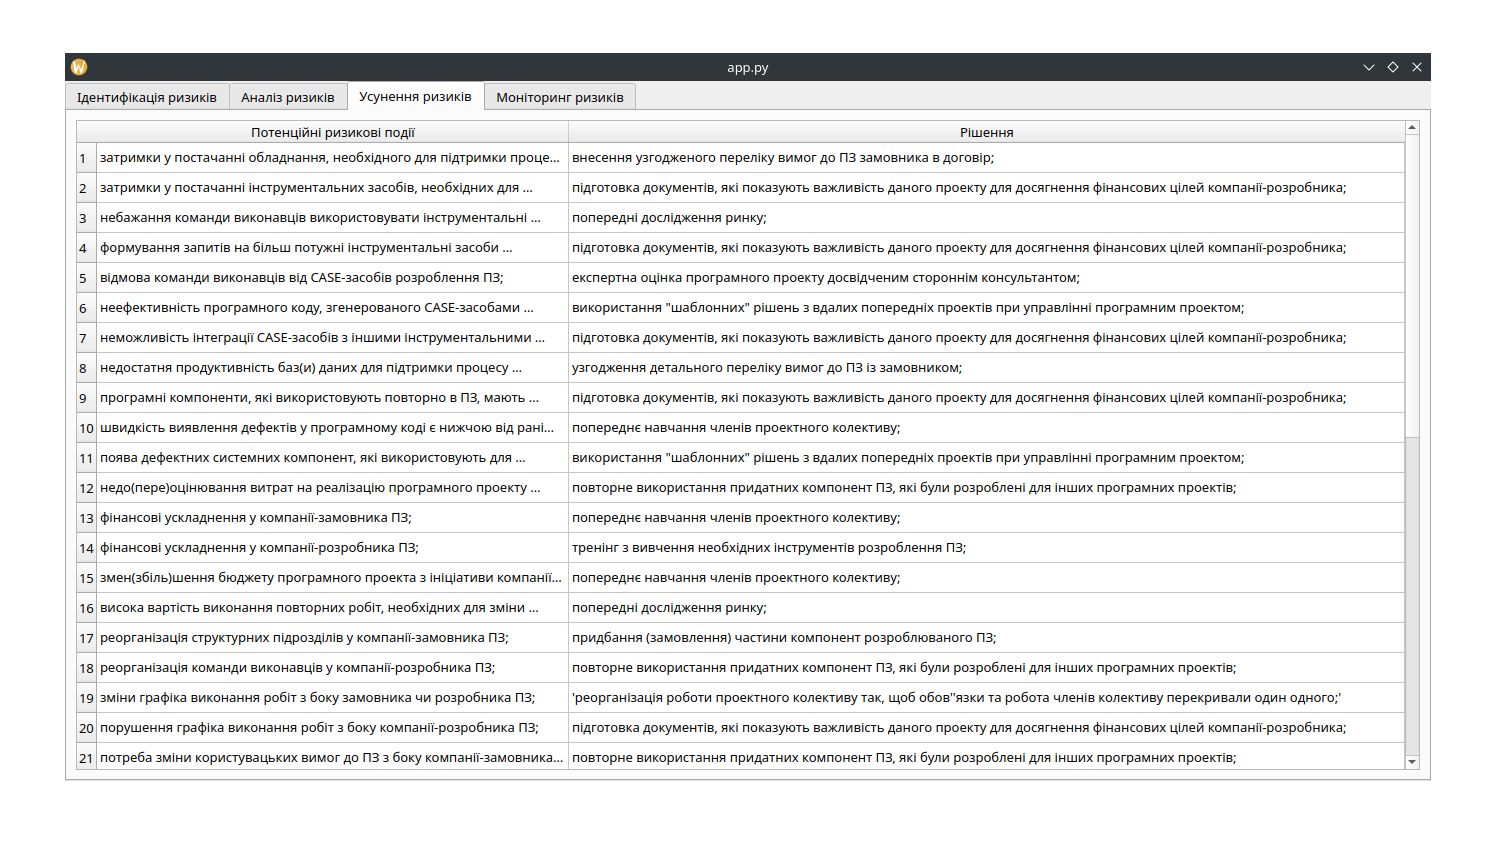
\includegraphics[scale=0.45]{5}
		\caption{Усунення ризиків}
	\end{figure}
	
	\begin{figure}[H]
		\centering
		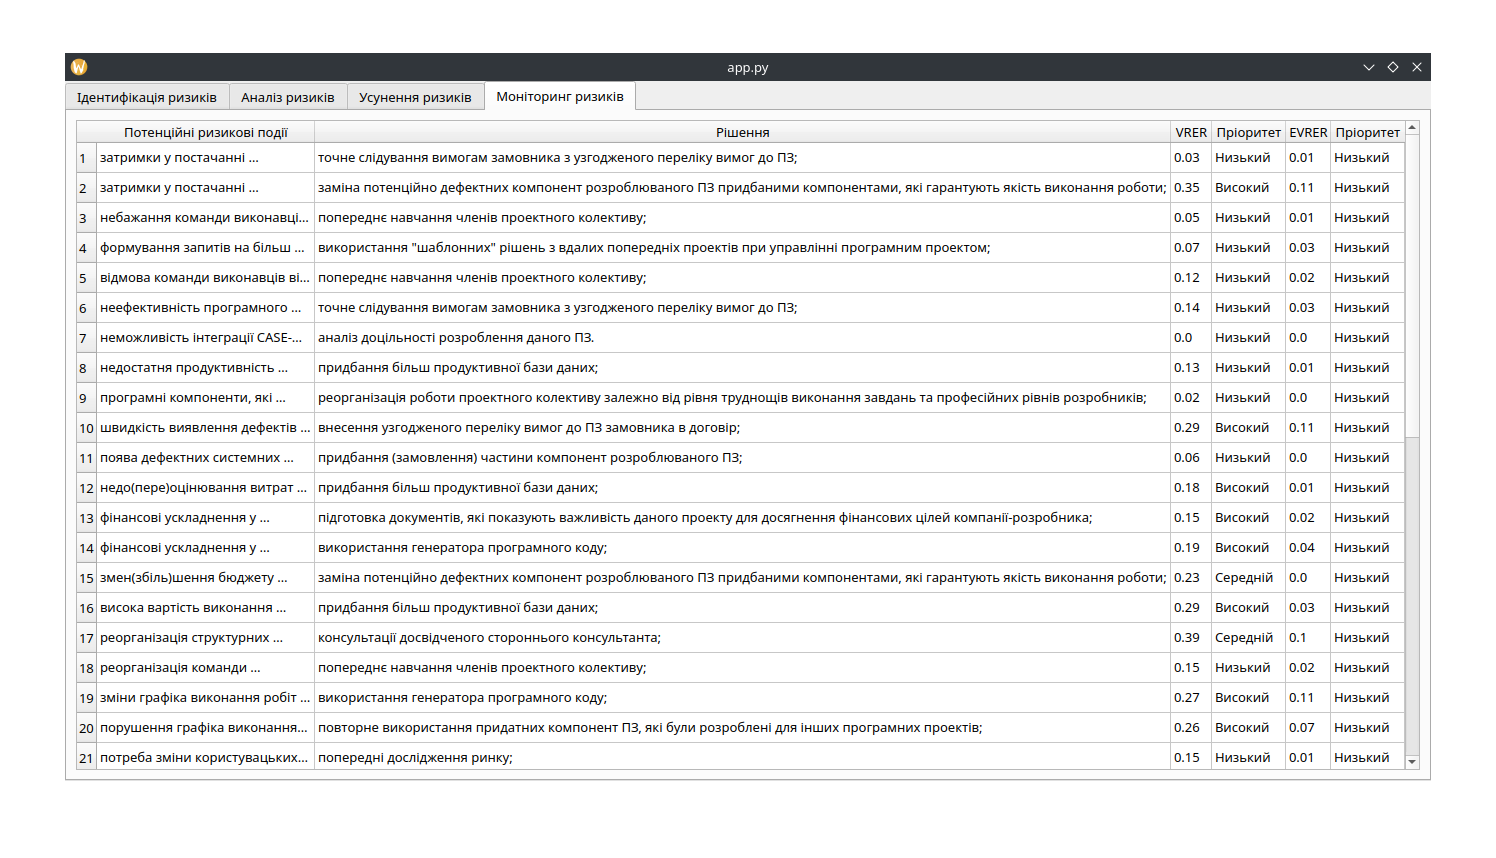
\includegraphics[scale=0.45]{6}
		\caption{Моніторинг ризиків}
	\end{figure}
	
	\section*{Висновок}
	Під час виконання лабораторної роботи я розробив програмне забезпечення за допомогою мови програмування Python та фреймворку PyQt6, яке дозволяє управляти ризиками розроблення ПЗ з використанням математичного методу. Програма характеризує всі деталі проходження етапів розроблення ризиків, а саме ідентифікацію, аналіз, що включає визначену величину ризику та ймовірність його появи, усунення та моніторинг, основною метою якого є оцінка використання заходів щодо зменшення впливу ризиків.
	
\end{normalsize}
\end{document}
